\documentclass[twoside]{book}

% Packages required by doxygen
\usepackage{fixltx2e}
\usepackage{calc}
\usepackage{doxygen}
\usepackage[export]{adjustbox} % also loads graphicx
\usepackage{graphicx}
\usepackage[utf8]{inputenc}
\usepackage{makeidx}
\usepackage{multicol}
\usepackage{multirow}
\PassOptionsToPackage{warn}{textcomp}
\usepackage{textcomp}
\usepackage[nointegrals]{wasysym}
\usepackage[table]{xcolor}

% Font selection
\usepackage[T1]{fontenc}
\usepackage[scaled=.90]{helvet}
\usepackage{courier}
\usepackage{amssymb}
\usepackage{sectsty}
\renewcommand{\familydefault}{\sfdefault}
\allsectionsfont{%
  \fontseries{bc}\selectfont%
  \color{darkgray}%
}
\renewcommand{\DoxyLabelFont}{%
  \fontseries{bc}\selectfont%
  \color{darkgray}%
}
\newcommand{\+}{\discretionary{\mbox{\scriptsize$\hookleftarrow$}}{}{}}

% Page & text layout
\usepackage{geometry}
\geometry{%
  a4paper,%
  top=2.5cm,%
  bottom=2.5cm,%
  left=2.5cm,%
  right=2.5cm%
}
\tolerance=750
\hfuzz=15pt
\hbadness=750
\setlength{\emergencystretch}{15pt}
\setlength{\parindent}{0cm}
\setlength{\parskip}{3ex plus 2ex minus 2ex}
\makeatletter
\renewcommand{\paragraph}{%
  \@startsection{paragraph}{4}{0ex}{-1.0ex}{1.0ex}{%
    \normalfont\normalsize\bfseries\SS@parafont%
  }%
}
\renewcommand{\subparagraph}{%
  \@startsection{subparagraph}{5}{0ex}{-1.0ex}{1.0ex}{%
    \normalfont\normalsize\bfseries\SS@subparafont%
  }%
}
\makeatother

% Headers & footers
\usepackage{fancyhdr}
\pagestyle{fancyplain}
\fancyhead[LE]{\fancyplain{}{\bfseries\thepage}}
\fancyhead[CE]{\fancyplain{}{}}
\fancyhead[RE]{\fancyplain{}{\bfseries\leftmark}}
\fancyhead[LO]{\fancyplain{}{\bfseries\rightmark}}
\fancyhead[CO]{\fancyplain{}{}}
\fancyhead[RO]{\fancyplain{}{\bfseries\thepage}}
\fancyfoot[LE]{\fancyplain{}{}}
\fancyfoot[CE]{\fancyplain{}{}}
\fancyfoot[RE]{\fancyplain{}{\bfseries\scriptsize Generated by Doxygen }}
\fancyfoot[LO]{\fancyplain{}{\bfseries\scriptsize Generated by Doxygen }}
\fancyfoot[CO]{\fancyplain{}{}}
\fancyfoot[RO]{\fancyplain{}{}}
\renewcommand{\footrulewidth}{0.4pt}
\renewcommand{\chaptermark}[1]{%
  \markboth{#1}{}%
}
\renewcommand{\sectionmark}[1]{%
  \markright{\thesection\ #1}%
}

% Indices & bibliography
\usepackage{natbib}
\usepackage[titles]{tocloft}
\setcounter{tocdepth}{3}
\setcounter{secnumdepth}{5}
\makeindex

% Hyperlinks (required, but should be loaded last)
\usepackage{ifpdf}
\ifpdf
  \usepackage[pdftex,pagebackref=true]{hyperref}
\else
  \usepackage[ps2pdf,pagebackref=true]{hyperref}
\fi
\hypersetup{%
  colorlinks=true,%
  linkcolor=blue,%
  citecolor=blue,%
  unicode%
}

% Custom commands
\newcommand{\clearemptydoublepage}{%
  \newpage{\pagestyle{empty}\cleardoublepage}%
}

\usepackage{caption}
\captionsetup{labelsep=space,justification=centering,font={bf},singlelinecheck=off,skip=4pt,position=top}

%===== C O N T E N T S =====

\begin{document}

% Titlepage & ToC
\hypersetup{pageanchor=false,
             bookmarksnumbered=true,
             pdfencoding=unicode
            }
\pagenumbering{alph}
\begin{titlepage}
\vspace*{7cm}
\begin{center}%
{\Large Stocks }\\
\vspace*{1cm}
{\large Generated by Doxygen 1.8.12}\\
\end{center}
\end{titlepage}
\clearemptydoublepage
\pagenumbering{roman}
\tableofcontents
\clearemptydoublepage
\pagenumbering{arabic}
\hypersetup{pageanchor=true}

%--- Begin generated contents ---
\chapter{Stock\+Forecast}
\label{md_README}
\hypertarget{md_README}{}
Basic framework for using a variety of models to forecast and simulate stock market performance.





\subsection*{To-\/\+Do}


\begin{DoxyItemize}
\item Switch getopt to argparse
\item Command line arguments for start and end dates
\item Neural network model
\item Add more performance metrics
\begin{DoxyItemize}
\item Good/\+Total predictions
\item Performance vs random
\item Portfolio improvement as function of stock improvement
\end{DoxyItemize}
\item Improve optimization code to avoid overfitting
\item Add makefile for doxygen, include profiling graph (code here until then)
\begin{DoxyItemize}
\item python -\/m c\+Profile -\/o logfile \hyperlink{stocks_8py}{stocks.\+py}
\item gprof2dot -\/f pstats logfile -\/o dotfile
\item dot dotfile -\/\+Tpng pngfile
\end{DoxyItemize}
\item Figure out why S\&P and D\+J\+IA seemingly observe different holidays
\item Make documentation more doxygen friendly
\end{DoxyItemize}

\subsection*{\href{docs/html/index.html}{\tt Doxygen documentation}}





\subsection*{History}


\begin{DoxyItemize}
\item \href{#april-4-2017}{\tt April 4\+: Initial Commit}
\end{DoxyItemize}

\subsubsection*{April 4, 2017}

Making the initial commit of this code to github. As it stands, the functionality ported over from my matlab stock framework is limited to linear and random models, but overall generalizability and functionality should be greatly expanded by using python. This also allows for installation on a server without another matlab license, which is nice.

Sample of the current state of predictions\+:

\tabulinesep=1mm
\begin{longtabu} spread 0pt [c]{*{2}{|X[-1]}|}
\hline
\rowcolor{\tableheadbgcolor}\PBS\centering {\bf \hyperlink{namespaceIR}{IR} Model }&\PBS\centering {\bf Randombuy Model  }\\\cline{1-2}
\endfirsthead
\hline
\endfoot
\hline
\rowcolor{\tableheadbgcolor}\PBS\centering {\bf \hyperlink{namespaceIR}{IR} Model }&\PBS\centering {\bf Randombuy Model  }\\\cline{1-2}
\endhead
\PBS\centering  &\PBS\centering  \\\cline{1-2}
\end{longtabu}
Working well at buying low and selling high short term, but definitely needs improvement in forecasting long term trends. Performance isn\textquotesingle{}t great for stocks in continual decline (which makes sense, except previous nonlinear models have set high expectations for being able to avoid this problem).

Also, just for fun, the profiler graph of a run\+:  
\chapter{Namespace Index}
\section{Namespace List}
Here is a list of all namespaces with brief descriptions\+:\begin{DoxyCompactList}
\item\contentsline{section}{\hyperlink{namespaceDecisionMethods}{Decision\+Methods} }{\pageref{namespaceDecisionMethods}}{}
\item\contentsline{section}{\hyperlink{namespaceIR}{IR} }{\pageref{namespaceIR}}{}
\item\contentsline{section}{\hyperlink{namespacestocks}{stocks} }{\pageref{namespacestocks}}{}
\end{DoxyCompactList}

\chapter{File Index}
\section{File List}
Here is a list of all files with brief descriptions\+:\begin{DoxyCompactList}
\item\contentsline{section}{\hyperlink{DecisionMethods_8py}{Decision\+Methods.\+py} }{\pageref{DecisionMethods_8py}}{}
\item\contentsline{section}{\hyperlink{IR_8py}{I\+R.\+py} }{\pageref{IR_8py}}{}
\item\contentsline{section}{\hyperlink{stocks_8py}{stocks.\+py} }{\pageref{stocks_8py}}{}
\end{DoxyCompactList}

\chapter{Namespace Documentation}
\hypertarget{namespaceDecisionMethods}{}\section{Decision\+Methods Namespace Reference}
\label{namespaceDecisionMethods}\index{Decision\+Methods@{Decision\+Methods}}
\subsection*{Functions}
\begin{DoxyCompactItemize}
\item 
def \hyperlink{namespaceDecisionMethods_a44bd5be577a4d99d6b2d144ad405dd09}{randombuy} (data, extra\+Arg)
\item 
def \hyperlink{namespaceDecisionMethods_aed1379cd4db8a24d6e5e45908a88cb4b}{weeklyrise} (data, extra\+Arg)
\item 
def \hyperlink{namespaceDecisionMethods_a4cb76bf4e82cc2509499af66f8c816b3}{dailyrise} (data, extra\+Arg)
\item 
def \hyperlink{namespaceDecisionMethods_a856437b184fc8efd2df5f7fe1ba3644d}{LS} (data, extra\+Arg)
\item 
def \hyperlink{namespaceDecisionMethods_a6ee6e338ea6a22bd13d5b9767b126f83}{I\+Rpred} (data, Nx=1, Nf=5, ratio=0.\+03, days=5, extra\+Arg)
\end{DoxyCompactItemize}


\subsection{Function Documentation}
\hypertarget{namespaceDecisionMethods_a4cb76bf4e82cc2509499af66f8c816b3}{}\label{namespaceDecisionMethods_a4cb76bf4e82cc2509499af66f8c816b3} 
\index{Decision\+Methods@{Decision\+Methods}!dailyrise@{dailyrise}}
\index{dailyrise@{dailyrise}!Decision\+Methods@{Decision\+Methods}}
\subsubsection{\texorpdfstring{dailyrise()}{dailyrise()}}
{\footnotesize\ttfamily def Decision\+Methods.\+dailyrise (\begin{DoxyParamCaption}\item[{}]{data,  }\item[{}]{extra\+Arg }\end{DoxyParamCaption})}



Definition at line 19 of file Decision\+Methods.\+py.



Referenced by stocks.\+simulate().


\begin{DoxyCode}
19 \textcolor{keyword}{def }\hyperlink{namespaceDecisionMethods_a4cb76bf4e82cc2509499af66f8c816b3}{dailyrise}(data,**extraArg):
20     difference=extraArg[\textcolor{stringliteral}{'difference'}]
21     if(data[-1]>data[-2]*(1+difference)):
22         \textcolor{keywordflow}{return} -1
23     elif(data[-1]<data[-2]*(1-difference)):
24         \textcolor{keywordflow}{return} 1
25     \textcolor{keywordflow}{else}:
26         \textcolor{keywordflow}{return} 0
27 
\end{DoxyCode}
\hypertarget{namespaceDecisionMethods_a6ee6e338ea6a22bd13d5b9767b126f83}{}\label{namespaceDecisionMethods_a6ee6e338ea6a22bd13d5b9767b126f83} 
\index{Decision\+Methods@{Decision\+Methods}!I\+Rpred@{I\+Rpred}}
\index{I\+Rpred@{I\+Rpred}!Decision\+Methods@{Decision\+Methods}}
\subsubsection{\texorpdfstring{I\+Rpred()}{IRpred()}}
{\footnotesize\ttfamily def Decision\+Methods.\+I\+Rpred (\begin{DoxyParamCaption}\item[{}]{data,  }\item[{}]{Nx = {\ttfamily 1},  }\item[{}]{Nf = {\ttfamily 5},  }\item[{}]{ratio = {\ttfamily 0.03},  }\item[{}]{days = {\ttfamily 5},  }\item[{}]{extra\+Arg }\end{DoxyParamCaption})}



Definition at line 48 of file Decision\+Methods.\+py.



Referenced by stocks.\+simulate().


\begin{DoxyCode}
48 \textcolor{keyword}{def }\hyperlink{namespaceDecisionMethods_a6ee6e338ea6a22bd13d5b9767b126f83}{IRpred}(data,Nx=1,Nf=5,ratio=0.03,days=5,**extraArg):
49     \textcolor{comment}{#Args: Nx, Nf, ratio, days}
50     X=data[1:,0]
51     F=data[:-1,1:]
52 
53     pred=\hyperlink{namespaceIR}{IR}(X,F,Nx,Nf)
54     if(pred>(X[-days-1]*(1+ratio))):
55         \textcolor{keywordflow}{return} -1
56     elif(pred<(X[-days-1]*(1-ratio))):
57         \textcolor{keywordflow}{return} 1
58     \textcolor{keywordflow}{else}:
59         \textcolor{keywordflow}{return} 0
60 
61     
62 \end{DoxyCode}
\hypertarget{namespaceDecisionMethods_a856437b184fc8efd2df5f7fe1ba3644d}{}\label{namespaceDecisionMethods_a856437b184fc8efd2df5f7fe1ba3644d} 
\index{Decision\+Methods@{Decision\+Methods}!LS@{LS}}
\index{LS@{LS}!Decision\+Methods@{Decision\+Methods}}
\subsubsection{\texorpdfstring{L\+S()}{LS()}}
{\footnotesize\ttfamily def Decision\+Methods.\+LS (\begin{DoxyParamCaption}\item[{}]{data,  }\item[{}]{extra\+Arg }\end{DoxyParamCaption})}



Definition at line 28 of file Decision\+Methods.\+py.



Referenced by stocks.\+simulate().


\begin{DoxyCode}
28 \textcolor{keyword}{def }\hyperlink{namespaceDecisionMethods_a856437b184fc8efd2df5f7fe1ba3644d}{LS}(data,**extraArg):
29     difference=extraArg[\textcolor{stringliteral}{'difference'}]
30     X=data[1:,0]
31     F=data[:-1,1:]
32     A=numpy.vstack([F.T,numpy.ones(len(X))]).T
33     m=numpy.linalg.lstsq(A,X)[0]
34     tomorrow=float(m[0]*F[-1]+m[1])
35 
36     logging.debug(\textcolor{stringliteral}{'X(end): \{0:.2f\}'}.format(X[-1]))
37     logging.debug(\textcolor{stringliteral}{'F(end): \{0:.2f\}'}.format(float(data[-1,1:])))
38     logging.debug(\textcolor{stringliteral}{'Tomorrow value: \{0:.2f\} from m: \{1:.2f\} c: \{2:.2f\}'}.format(tomorrow,m[0],m[1]))
39 
40     if(tomorrow>X[-1]*(1+difference)):
41         \textcolor{keywordflow}{return} -1
42     elif(tomorrow<X[-1]*(1-difference)):
43         \textcolor{keywordflow}{return} 1
44     \textcolor{keywordflow}{else}:
45         \textcolor{keywordflow}{return} 0
46 
47 
\end{DoxyCode}
\hypertarget{namespaceDecisionMethods_a44bd5be577a4d99d6b2d144ad405dd09}{}\label{namespaceDecisionMethods_a44bd5be577a4d99d6b2d144ad405dd09} 
\index{Decision\+Methods@{Decision\+Methods}!randombuy@{randombuy}}
\index{randombuy@{randombuy}!Decision\+Methods@{Decision\+Methods}}
\subsubsection{\texorpdfstring{randombuy()}{randombuy()}}
{\footnotesize\ttfamily def Decision\+Methods.\+randombuy (\begin{DoxyParamCaption}\item[{}]{data,  }\item[{}]{extra\+Arg }\end{DoxyParamCaption})}



Definition at line 6 of file Decision\+Methods.\+py.



Referenced by stocks.\+simulate().


\begin{DoxyCode}
6 \textcolor{keyword}{def }\hyperlink{namespaceDecisionMethods_a44bd5be577a4d99d6b2d144ad405dd09}{randombuy}(data,**extraArg):
7     \textcolor{keywordflow}{return} randint(-1,1)
8 
\end{DoxyCode}
\hypertarget{namespaceDecisionMethods_aed1379cd4db8a24d6e5e45908a88cb4b}{}\label{namespaceDecisionMethods_aed1379cd4db8a24d6e5e45908a88cb4b} 
\index{Decision\+Methods@{Decision\+Methods}!weeklyrise@{weeklyrise}}
\index{weeklyrise@{weeklyrise}!Decision\+Methods@{Decision\+Methods}}
\subsubsection{\texorpdfstring{weeklyrise()}{weeklyrise()}}
{\footnotesize\ttfamily def Decision\+Methods.\+weeklyrise (\begin{DoxyParamCaption}\item[{}]{data,  }\item[{}]{extra\+Arg }\end{DoxyParamCaption})}



Definition at line 9 of file Decision\+Methods.\+py.


\begin{DoxyCode}
9 \textcolor{keyword}{def }\hyperlink{namespaceDecisionMethods_aed1379cd4db8a24d6e5e45908a88cb4b}{weeklyrise}(data,**extraArg):
10     difference=extraArg[\textcolor{stringliteral}{'difference'}]
11     if(data[-1]>data[-6]*(1+difference)):
12         \textcolor{keywordflow}{return} -1
13     elif(data[-1]<data[-6]*(1-difference)):
14         \textcolor{keywordflow}{return} 1
15     \textcolor{keywordflow}{else}:
16         \textcolor{keywordflow}{return} 0
17 
18 
\end{DoxyCode}

\hypertarget{namespaceIR}{}\section{IR Namespace Reference}
\label{namespaceIR}\index{IR@{IR}}
\subsection*{Functions}
\begin{DoxyCompactItemize}
\item 
def \hyperlink{namespaceIR_ae50bbbd323bc928d9e274617de58d72f}{IR} (X, F, Nx, Nf)
\item 
def \hyperlink{namespaceIR_aeaee615025a0b0c13500382312ba7745}{verify\+IR} ()
\end{DoxyCompactItemize}


\subsection{Function Documentation}
\hypertarget{namespaceIR_ae50bbbd323bc928d9e274617de58d72f}{}\label{namespaceIR_ae50bbbd323bc928d9e274617de58d72f} 
\index{IR@{IR}!IR@{IR}}
\index{IR@{IR}!IR@{IR}}
\subsubsection{\texorpdfstring{I\+R()}{IR()}}
{\footnotesize\ttfamily def I\+R.\+IR (\begin{DoxyParamCaption}\item[{}]{X,  }\item[{}]{F,  }\item[{}]{Nx,  }\item[{}]{Nf }\end{DoxyParamCaption})}



Definition at line 4 of file I\+R.\+py.


\begin{DoxyCode}
4 \textcolor{keyword}{def }\hyperlink{namespaceIR_ae50bbbd323bc928d9e274617de58d72f}{IR}(X,F,Nx,Nf):
5     \textcolor{comment}{#Define what indices prediction should start on}
6     predstart=max(Nx,Nf)
7 
8     xstart=predstart-Nx
9     fstart=predstart-Nf
10 
11     \textcolor{comment}{#print("pred: \{\} xs \{\} fs \{\}".format(predstart,xstart,fstart))}
12     matlen=len(X)-predstart
13 
14     Nimpulses=min(np.shape(F))
15 
16     \textcolor{comment}{#Initialize matrix to solve.}
17     Z=np.zeros((matlen,Nx+Nf*Nimpulses+1))
18     \textcolor{comment}{#Matrix for predicting next value using last of data}
19     PredZ=np.zeros(Nx+Nf*Nimpulses+1)
20 
21     \textcolor{keywordflow}{for} i \textcolor{keywordflow}{in} range(0,Nx):
22         Z[:,i]=X[xstart+i:xstart+i+matlen]
23         PredZ[i]=X[len(X)-Nx+i]
24     \textcolor{keywordflow}{for} i \textcolor{keywordflow}{in} range(0,Nf):
25         \textcolor{keywordflow}{for} j \textcolor{keywordflow}{in} range(0,Nimpulses):
26             Z[:,(i+Nx+j*Nf)]=F[(fstart+i):(fstart+i+matlen),j]
27             PredZ[i+Nx+j*Nf]=F[len(X)-Nf+i,j]
28 
29     Z[:,-1]=np.ones(matlen)
30     PredZ[-1]=1
31     B=X[predstart:(predstart+matlen),\textcolor{keywordtype}{None}]
32 
33     Z=np.hstack([Z,B])
34 
35     delmask=np.all(np.isnan(Z), axis=1)
36     Z=Z[~delmask]
37 
38     B=Z[:,-1]
39     A=Z[:,:-1]
40 
41     m = np.linalg.lstsq(A,B)[0]
42     \textcolor{keywordflow}{return} np.dot(PredZ,m)
43 
44 
\end{DoxyCode}
\hypertarget{namespaceIR_aeaee615025a0b0c13500382312ba7745}{}\label{namespaceIR_aeaee615025a0b0c13500382312ba7745} 
\index{IR@{IR}!verify\+IR@{verify\+IR}}
\index{verify\+IR@{verify\+IR}!IR@{IR}}
\subsubsection{\texorpdfstring{verify\+I\+R()}{verifyIR()}}
{\footnotesize\ttfamily def I\+R.\+verify\+IR (\begin{DoxyParamCaption}{ }\end{DoxyParamCaption})}



Definition at line 45 of file I\+R.\+py.


\begin{DoxyCode}
45 \textcolor{keyword}{def }\hyperlink{namespaceIR_aeaee615025a0b0c13500382312ba7745}{verifyIR}():
46     F=np.random.rand(100,2)
47     X=np.arange(0.0,100.0,1.0)
48     F[:,0]=np.arange(0.0,100.0,1.0)
49     \textcolor{keywordflow}{for} i \textcolor{keywordflow}{in} range(2,100):
50         X[i]=F[i-2,0]*0.4+F[i-1,0]*0.6+0.3
51 
52     pred=\hyperlink{namespaceIR}{IR}(X,F,2,2)
53     print(pred)
54 
55     F=np.random.rand(100,2)
56     \textcolor{comment}{#X=np.arange(0.0,100.0,1.0)}
57     X=np.squeeze(np.random.rand(100,1))
58 
59     \textcolor{keywordflow}{for} i \textcolor{keywordflow}{in} range(1,100):
60         X[i]=X[i-1]*0.4+X[i-2]*0.2-F[i-1,0]*0.6+F[i-1,1]*0.2+0.5
61 
62 
63     pred=\hyperlink{namespaceIR}{IR}(X,F,2,3)
64     print(pred)
65 
66 
67 
68 \textcolor{stringliteral}{'''}
69 \textcolor{stringliteral}{def main(argv):}
70 \textcolor{stringliteral}{    F=np.random.rand(100,2)}
71 \textcolor{stringliteral}{    X=np.arange(0.0,100.0,1.0)}
72 \textcolor{stringliteral}{    F[:,0]=np.arange(0.0,100.0,1.0)}
73 \textcolor{stringliteral}{    for i in range(2,100):}
74 \textcolor{stringliteral}{        X[i]=F[i-2,0]*0.4+F[i-1,0]*0.6+0.3}
75 \textcolor{stringliteral}{}
76 \textcolor{stringliteral}{    pred=IR(X,F,2,2)}
77 \textcolor{stringliteral}{    print(pred)}
78 \textcolor{stringliteral}{}
79 \textcolor{stringliteral}{}
80 \textcolor{stringliteral}{if \_\_name\_\_ == "\_\_main\_\_":}
81 \textcolor{stringliteral}{    main(sys.argv)}
82 \textcolor{stringliteral}{'''}
83 \end{DoxyCode}

\hypertarget{namespacestocks}{}\section{stocks Namespace Reference}
\label{namespacestocks}\index{stocks@{stocks}}
\subsection*{Functions}
\begin{DoxyCompactItemize}
\item 
def \hyperlink{namespacestocks_a44235135cad9d919663b15452cf3e613}{get\+Closing} (Tick, start=str(date(date.\+today().year-\/1, date.\+today().month, date.\+today().day)), end=str(date.\+today()))
\item 
def \hyperlink{namespacestocks_a6217dcad564ba6361c3cca44542ba220}{simulate} (simtype, amount, data, return\+Series=0, plot=0, extra\+Arg)
\item 
def \hyperlink{namespacestocks_ac80b7d5d1cdc027b7a0e2e19093baf9b}{result\+Print} (method, ticker, start, end)
\item 
def \hyperlink{namespacestocks_a7d4f88b285b7a553f17f91e71ee18a31}{ensemble\+Sim} (simtype, starting\+Worth, data, ticker, ensemble\+Num=100, extra\+Arg)
\item 
def \hyperlink{namespacestocks_a5ce0ea6dd1cb1e1baf78fbb4313b64b9}{Common\+Date} (dateX, X, dateF, F)
\item 
def \hyperlink{namespacestocks_a001673a0b7e5f0867197d97fea8a251b}{Optimize\+IR} (data, starting\+Worth, extra\+Arg)
\item 
def \hyperlink{namespacestocks_aa4d6e539aeea3ab00b8bf598b1025e58}{main} (argv)
\end{DoxyCompactItemize}


\subsection{Function Documentation}
\hypertarget{namespacestocks_a5ce0ea6dd1cb1e1baf78fbb4313b64b9}{}\label{namespacestocks_a5ce0ea6dd1cb1e1baf78fbb4313b64b9} 
\index{stocks@{stocks}!Common\+Date@{Common\+Date}}
\index{Common\+Date@{Common\+Date}!stocks@{stocks}}
\subsubsection{\texorpdfstring{Common\+Date()}{CommonDate()}}
{\footnotesize\ttfamily def stocks.\+Common\+Date (\begin{DoxyParamCaption}\item[{}]{dateX,  }\item[{}]{X,  }\item[{}]{dateF,  }\item[{}]{F }\end{DoxyParamCaption})}



Definition at line 153 of file stocks.\+py.



Referenced by main().


\begin{DoxyCode}
153 \textcolor{keyword}{def }\hyperlink{namespacestocks_a5ce0ea6dd1cb1e1baf78fbb4313b64b9}{CommonDate}(dateX,X,dateF,F):
154     Xdic=dict(zip(dateX,X))
155     Fdic=dict(zip(dateF,F))
156     common=(Xdic.keys() & Fdic.keys())
157     F=[Fdic[i] \textcolor{keywordflow}{for} i \textcolor{keywordflow}{in} sorted(common)]
158     \textcolor{keywordflow}{return} F
159 
\end{DoxyCode}
\hypertarget{namespacestocks_a7d4f88b285b7a553f17f91e71ee18a31}{}\label{namespacestocks_a7d4f88b285b7a553f17f91e71ee18a31} 
\index{stocks@{stocks}!ensemble\+Sim@{ensemble\+Sim}}
\index{ensemble\+Sim@{ensemble\+Sim}!stocks@{stocks}}
\subsubsection{\texorpdfstring{ensemble\+Sim()}{ensembleSim()}}
{\footnotesize\ttfamily def stocks.\+ensemble\+Sim (\begin{DoxyParamCaption}\item[{}]{simtype,  }\item[{}]{starting\+Worth,  }\item[{}]{data,  }\item[{}]{ticker,  }\item[{}]{ensemble\+Num = {\ttfamily 100},  }\item[{}]{extra\+Arg }\end{DoxyParamCaption})}

\begin{DoxyVerb}Run a model a number of times, look at median results
Not sure if it technically counts as an "ensemble" model, but
good way to observe effects of random variations in models that
have random variations
\end{DoxyVerb}
 

Definition at line 124 of file stocks.\+py.



References simulate().



Referenced by main().


\begin{DoxyCode}
124 \textcolor{keyword}{def }\hyperlink{namespacestocks_a7d4f88b285b7a553f17f91e71ee18a31}{ensembleSim}(simtype, startingWorth, data, ticker, ensembleNum=100, **extraArg):
125     \textcolor{stringliteral}{'''Run a model a number of times, look at median results}
126 \textcolor{stringliteral}{    Not sure if it technically counts as an "ensemble" model, but}
127 \textcolor{stringliteral}{    good way to observe effects of random variations in models that}
128 \textcolor{stringliteral}{    have random variations}
129 \textcolor{stringliteral}{    '''}
130 
131     ensembleRun=np.zeros([ensembleNum,len(\hyperlink{namespacestocks_a6217dcad564ba6361c3cca44542ba220}{simulate}(simtype,startingWorth,data,**extraArg,
      returnSeries=1))])
132     \textcolor{keywordflow}{for} run \textcolor{keywordflow}{in} range(ensembleNum):
133         ensembleRun[run,:] = \hyperlink{namespacestocks_a6217dcad564ba6361c3cca44542ba220}{simulate}(simtype,startingWorth,data,**extraArg,returnSeries=1)
134 
135 
136     ensMed=np.median(ensembleRun,0)
137 
138     date=extraArg.get(\textcolor{stringliteral}{'date'},[i \textcolor{keywordflow}{for} i \textcolor{keywordflow}{in} range(len(ensMed))])
139 
140 
141     plt.plot(date,ensMed, \textcolor{stringliteral}{'k'})
142     plt.plot(date,[startingWorth \textcolor{keywordflow}{for} i \textcolor{keywordflow}{in} range(len(ensMed))],\textcolor{stringliteral}{'r-.'})
143 
144     plt.fill\_between(date,ensMed-2.0*np.std(ensembleRun,0), ensMed+2.0*np.std(ensembleRun,0), color=\textcolor{stringliteral}{'b'}, 
      alpha=0.2)
145 
146     plt.ylabel(\textcolor{stringliteral}{'Value ($)'})
147     plt.xlabel(\textcolor{stringliteral}{'Date'})
148     plt.title(\textcolor{stringliteral}{'Simulating use of \{\} for \{\}'}.format(simtype.\_\_name\_\_,ticker))
149     plt.savefig(\textcolor{stringliteral}{'Plots/\{\}\_\{\}\_ensemble.png'}.format(ticker,simtype.\_\_name\_\_))
150     plt.show()
151 
152 
\end{DoxyCode}
Here is the call graph for this function\+:\nopagebreak
\begin{figure}[H]
\begin{center}
\leavevmode
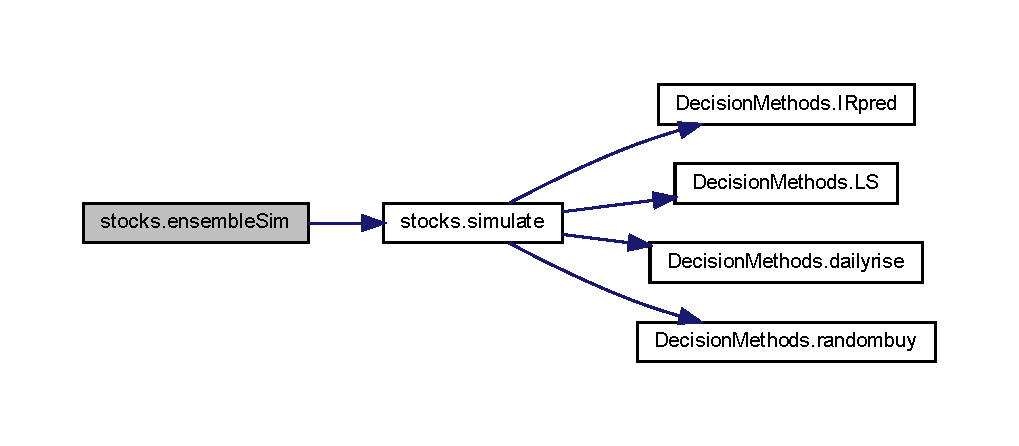
\includegraphics[width=350pt]{namespacestocks_a7d4f88b285b7a553f17f91e71ee18a31_cgraph}
\end{center}
\end{figure}
\hypertarget{namespacestocks_a44235135cad9d919663b15452cf3e613}{}\label{namespacestocks_a44235135cad9d919663b15452cf3e613} 
\index{stocks@{stocks}!get\+Closing@{get\+Closing}}
\index{get\+Closing@{get\+Closing}!stocks@{stocks}}
\subsubsection{\texorpdfstring{get\+Closing()}{getClosing()}}
{\footnotesize\ttfamily def stocks.\+get\+Closing (\begin{DoxyParamCaption}\item[{}]{Tick,  }\item[{}]{start = {\ttfamily str(date(date.today().year-\/1,date.today().month,date.today().day))},  }\item[{}]{end = {\ttfamily str(date.today())} }\end{DoxyParamCaption})}



Definition at line 14 of file stocks.\+py.



Referenced by main().


\begin{DoxyCode}
14 \textcolor{keyword}{def }\hyperlink{namespacestocks_a44235135cad9d919663b15452cf3e613}{getClosing}(Tick,start=str(date(date.today().year-1,date.today().month,date.today().day)),end=
      str(date.today())):
15     stock = Share(Tick)
16     stockhist=stock.get\_historical(start,end)
17 
18     vals=list()
19     vals=[float(stockhist[i][\textcolor{stringliteral}{'Close'}]) \textcolor{keywordflow}{for} i \textcolor{keywordflow}{in} range(len(stockhist))]
20     dates=[datetime.datetime.strptime(stockhist[i][\textcolor{stringliteral}{'Date'}],\textcolor{stringliteral}{'%Y-%m-%d'}) \textcolor{keywordflow}{for} i \textcolor{keywordflow}{in} range(len(stockhist))]
21 
22     \textcolor{keywordflow}{return} (dates,vals)
23 
24 
25 
\end{DoxyCode}
\hypertarget{namespacestocks_aa4d6e539aeea3ab00b8bf598b1025e58}{}\label{namespacestocks_aa4d6e539aeea3ab00b8bf598b1025e58} 
\index{stocks@{stocks}!main@{main}}
\index{main@{main}!stocks@{stocks}}
\subsubsection{\texorpdfstring{main()}{main()}}
{\footnotesize\ttfamily def stocks.\+main (\begin{DoxyParamCaption}\item[{}]{argv }\end{DoxyParamCaption})}



Definition at line 178 of file stocks.\+py.



References Common\+Date(), ensemble\+Sim(), get\+Closing(), result\+Print(), and simulate().


\begin{DoxyCode}
178 \textcolor{keyword}{def }\hyperlink{namespacestocks_aa4d6e539aeea3ab00b8bf598b1025e58}{main}(argv):
179     opts, args = getopt.getopt(argv[1:],\textcolor{stringliteral}{"hlt:"},[\textcolor{stringliteral}{"log="},\textcolor{stringliteral}{"ticker="}])
180     \textcolor{keywordflow}{for} opt, arg \textcolor{keywordflow}{in} opts:
181         \textcolor{keywordflow}{if} opt==\textcolor{stringliteral}{"-h"}:
182             print(\textcolor{stringliteral}{'python read.py'})
183         \textcolor{keywordflow}{elif} opt \textcolor{keywordflow}{in} (\textcolor{stringliteral}{"-l"},\textcolor{stringliteral}{"--log"}):
184             loglevel=arg
185         \textcolor{keywordflow}{elif} opt \textcolor{keywordflow}{in} (\textcolor{stringliteral}{"-t"},\textcolor{stringliteral}{"--ticker"}):
186             ticker=arg
187 
188     if(\textcolor{stringliteral}{'ticker'} \textcolor{keywordflow}{not} \textcolor{keywordflow}{in} vars()):
189         ticker = \textcolor{stringliteral}{'ABX'}
190     if(\textcolor{stringliteral}{'loglevel'} \textcolor{keywordflow}{not} \textcolor{keywordflow}{in} vars()):
191         loglevel=\textcolor{stringliteral}{'WARNING'}
192 
193     logging.basicConfig(format=\textcolor{stringliteral}{'%(levelname)s:%(message)s'},level=loglevel)
194 
195     (dateX,X)=\hyperlink{namespacestocks_a44235135cad9d919663b15452cf3e613}{getClosing}(ticker)
196     \textcolor{comment}{#Because this somehow gets reversed}
197     dateX.sort()
198 
199     startingWorth=10000
200     \hyperlink{namespacestocks_ac80b7d5d1cdc027b7a0e2e19093baf9b}{resultPrint}(\textcolor{stringliteral}{'Randombuy'},ticker,startingWorth,\hyperlink{namespacestocks_a6217dcad564ba6361c3cca44542ba220}{simulate}(randombuy,startingWorth,X))
201     \hyperlink{namespacestocks_ac80b7d5d1cdc027b7a0e2e19093baf9b}{resultPrint}(\textcolor{stringliteral}{'Weekbuy'},ticker,startingWorth,\hyperlink{namespacestocks_a6217dcad564ba6361c3cca44542ba220}{simulate}(weeklyrise,startingWorth,X,
      difference=0.1))
202     \hyperlink{namespacestocks_ac80b7d5d1cdc027b7a0e2e19093baf9b}{resultPrint}(\textcolor{stringliteral}{'Dailybuy'},ticker,startingWorth,\hyperlink{namespacestocks_a6217dcad564ba6361c3cca44542ba220}{simulate}(dailyrise,startingWorth,X,
      difference=0.05))
203 
204     \textcolor{comment}{#Get extra variables and strip them to times that exist with X}
205     (dateF,F)=\hyperlink{namespacestocks_a44235135cad9d919663b15452cf3e613}{getClosing}(\textcolor{stringliteral}{'^DJI'})
206     (dateF2, F2)=\hyperlink{namespacestocks_a44235135cad9d919663b15452cf3e613}{getClosing}(\textcolor{stringliteral}{'^GSPC'})
207     (dateF3, F3)=\hyperlink{namespacestocks_a44235135cad9d919663b15452cf3e613}{getClosing}(\textcolor{stringliteral}{'^IXIC'})
208     (dateF4, F4)=\hyperlink{namespacestocks_a44235135cad9d919663b15452cf3e613}{getClosing}(\textcolor{stringliteral}{'GE'})
209     F=\hyperlink{namespacestocks_a5ce0ea6dd1cb1e1baf78fbb4313b64b9}{CommonDate}(dateX,X,dateF,F)
210     \textcolor{comment}{#F=np.random.randn(1,len(F)).tolist()[0]}
211     F2=\hyperlink{namespacestocks_a5ce0ea6dd1cb1e1baf78fbb4313b64b9}{CommonDate}(dateX,X,dateF2,F2)
212     F3=\hyperlink{namespacestocks_a5ce0ea6dd1cb1e1baf78fbb4313b64b9}{CommonDate}(dateX,X,dateF3,F3)
213     F4=\hyperlink{namespacestocks_a5ce0ea6dd1cb1e1baf78fbb4313b64b9}{CommonDate}(dateX,X,dateF4,F4)
214 
215 
216     \hyperlink{namespacestocks_ac80b7d5d1cdc027b7a0e2e19093baf9b}{resultPrint}(\textcolor{stringliteral}{'LS'},ticker,startingWorth,\hyperlink{namespacestocks_a6217dcad564ba6361c3cca44542ba220}{simulate}(LS,startingWorth,np.array([X,F]).T,
      difference=0.05))
217     \hyperlink{namespacestocks_ac80b7d5d1cdc027b7a0e2e19093baf9b}{resultPrint}(\textcolor{stringliteral}{'IR'},ticker,startingWorth,\hyperlink{namespacestocks_a6217dcad564ba6361c3cca44542ba220}{simulate}(IRpred,startingWorth,np.array([X,F]).
      T,Nx=1,Nf=7,ratio=0.03,days=5))
218     \hyperlink{namespacestocks_ac80b7d5d1cdc027b7a0e2e19093baf9b}{resultPrint}(\textcolor{stringliteral}{'IR2'},ticker,startingWorth,\hyperlink{namespacestocks_a6217dcad564ba6361c3cca44542ba220}{simulate}(IRpred,startingWorth,np.array([X,F,
      F2]).T,Nx=1,Nf=7,ratio=0.03,days=5))
219     \hyperlink{namespacestocks_ac80b7d5d1cdc027b7a0e2e19093baf9b}{resultPrint}(\textcolor{stringliteral}{'IR3'},ticker,startingWorth,\hyperlink{namespacestocks_a6217dcad564ba6361c3cca44542ba220}{simulate}(IRpred,startingWorth,np.array([X,F,
      F2,F3]).T,Nx=1,Nf=7,ratio=0.03,days=5))
220     \hyperlink{namespacestocks_ac80b7d5d1cdc027b7a0e2e19093baf9b}{resultPrint}(\textcolor{stringliteral}{'IR4'},ticker,startingWorth,\hyperlink{namespacestocks_a6217dcad564ba6361c3cca44542ba220}{simulate}(IRpred,startingWorth,np.array([X,F,
      F2,F3,F4]).T,Nx=1,Nf=7,ratio=0.03,days=5))
221     \hyperlink{namespacestocks_ac80b7d5d1cdc027b7a0e2e19093baf9b}{resultPrint}(\textcolor{stringliteral}{'IR5'},ticker,startingWorth,\hyperlink{namespacestocks_a6217dcad564ba6361c3cca44542ba220}{simulate}(IRpred,startingWorth,np.array([X,F,
      F4]).T,Nx=1,Nf=7,ratio=0.03,days=5))
222 
223 
224 
225     \textcolor{comment}{#Simulate and plot ensemble  model. Only really useful for models with random/variable component}
226     \hyperlink{namespacestocks_a7d4f88b285b7a553f17f91e71ee18a31}{ensembleSim}(randombuy,startingWorth,np.array([X,F]).T,ticker)
227 
228     \hyperlink{namespacestocks_a6217dcad564ba6361c3cca44542ba220}{simulate}(IRpred,startingWorth,np.array([X,F]).T,Nx=1,Nf=7,ratio=0.03,days=5,plot=1,ticker=
      ticker,date=dateX)
229     \hyperlink{namespacestocks_a6217dcad564ba6361c3cca44542ba220}{simulate}(IRpred,startingWorth,np.array([X,F,F2]).T,Nx=1,Nf=7,ratio=0.03,days=5,plot=1,ticker=
      ticker,date=dateX)
230 
231     \textcolor{comment}{#OptimizeIR(np.array([X,F]).T,startingWorth,Nx=1,Nf=2,ratio=0.03,days=6, ticker=ticker)}
232 
233 
\end{DoxyCode}
Here is the call graph for this function\+:\nopagebreak
\begin{figure}[H]
\begin{center}
\leavevmode
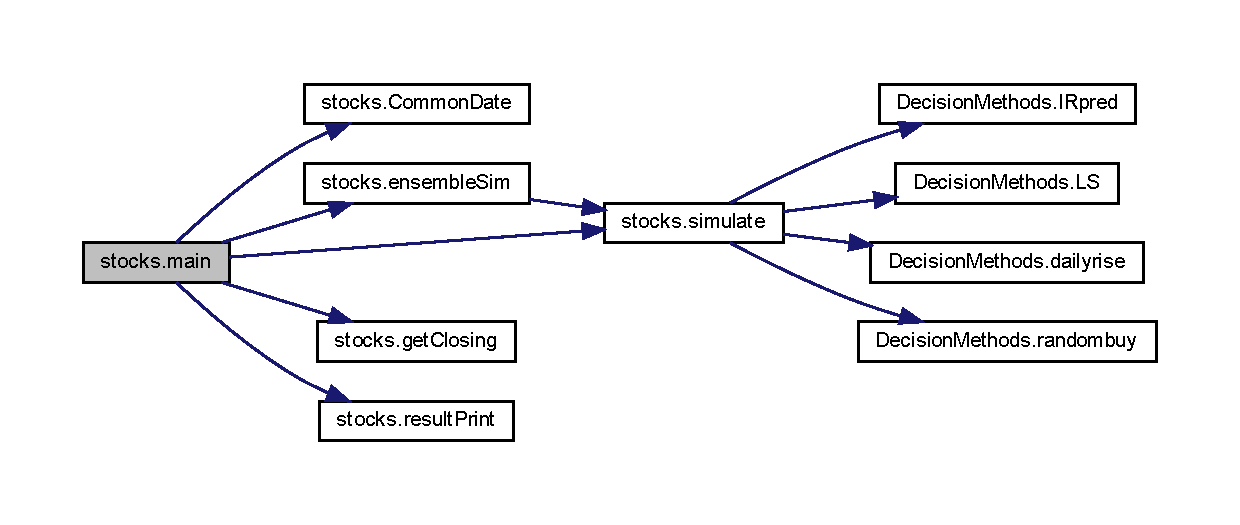
\includegraphics[width=350pt]{namespacestocks_aa4d6e539aeea3ab00b8bf598b1025e58_cgraph}
\end{center}
\end{figure}
\hypertarget{namespacestocks_a001673a0b7e5f0867197d97fea8a251b}{}\label{namespacestocks_a001673a0b7e5f0867197d97fea8a251b} 
\index{stocks@{stocks}!Optimize\+IR@{Optimize\+IR}}
\index{Optimize\+IR@{Optimize\+IR}!stocks@{stocks}}
\subsubsection{\texorpdfstring{Optimize\+I\+R()}{OptimizeIR()}}
{\footnotesize\ttfamily def stocks.\+Optimize\+IR (\begin{DoxyParamCaption}\item[{}]{data,  }\item[{}]{starting\+Worth,  }\item[{}]{extra\+Arg }\end{DoxyParamCaption})}



Definition at line 160 of file stocks.\+py.



References result\+Print(), and simulate().


\begin{DoxyCode}
160 \textcolor{keyword}{def }\hyperlink{namespacestocks_a001673a0b7e5f0867197d97fea8a251b}{OptimizeIR}(data,startingWorth,**extraArg):
161     Nx=extraArg.get(\textcolor{stringliteral}{'Nx'},1)
162     Nf=extraArg.get(\textcolor{stringliteral}{'Nf'},5)
163     ratio=extraArg.get(\textcolor{stringliteral}{'ratio'},0.03)
164     days=extraArg.get(\textcolor{stringliteral}{'days'},5)
165     ticker=extraArg.get(\textcolor{stringliteral}{'ticker'},\textcolor{stringliteral}{'ABX'})
166     \textcolor{comment}{#simulate(IRpred,start,data,Nx=Nx,Nf=Nf,ratio=ratio,days=days)}
167     \textcolor{keywordflow}{for} Nxtry \textcolor{keywordflow}{in} range(0,10):
168         \hyperlink{namespacestocks_ac80b7d5d1cdc027b7a0e2e19093baf9b}{resultPrint}(\textcolor{stringliteral}{'IR - Nx \{\}'}.format(Nxtry),ticker,startingWorth,
      \hyperlink{namespacestocks_a6217dcad564ba6361c3cca44542ba220}{simulate}(IRpred,startingWorth,data,Nx=Nxtry,Nf=Nf,ratio=ratio,days=days))
169     \textcolor{keywordflow}{for} Nftry \textcolor{keywordflow}{in} range(0,10):
170         \hyperlink{namespacestocks_ac80b7d5d1cdc027b7a0e2e19093baf9b}{resultPrint}(\textcolor{stringliteral}{'IR - Nf \{\}'}.format(Nftry),ticker,startingWorth,
      \hyperlink{namespacestocks_a6217dcad564ba6361c3cca44542ba220}{simulate}(IRpred,startingWorth,data,Nx=Nx,Nf=Nftry,ratio=ratio,days=days))
171     \textcolor{keywordflow}{for} ratiotry \textcolor{keywordflow}{in} np.arange(0.0,0.1,0.01):
172         \hyperlink{namespacestocks_ac80b7d5d1cdc027b7a0e2e19093baf9b}{resultPrint}(\textcolor{stringliteral}{'IR - ratio \{\}'}.format(ratiotry),ticker,startingWorth,
      \hyperlink{namespacestocks_a6217dcad564ba6361c3cca44542ba220}{simulate}(IRpred,startingWorth,data,Nx=Nx,Nf=Nf,ratio=ratiotry,days=days))
173     \textcolor{keywordflow}{for} daystry \textcolor{keywordflow}{in} [1,5,6,10,12,15]:
174         \hyperlink{namespacestocks_ac80b7d5d1cdc027b7a0e2e19093baf9b}{resultPrint}(\textcolor{stringliteral}{'IR - days \{\}'}.format(daystry),ticker,startingWorth,
      \hyperlink{namespacestocks_a6217dcad564ba6361c3cca44542ba220}{simulate}(IRpred,startingWorth,data,Nx=Nx,Nf=Nf,ratio=ratio,days=daystry))
175 
176 
177 
\end{DoxyCode}
Here is the call graph for this function\+:\nopagebreak
\begin{figure}[H]
\begin{center}
\leavevmode
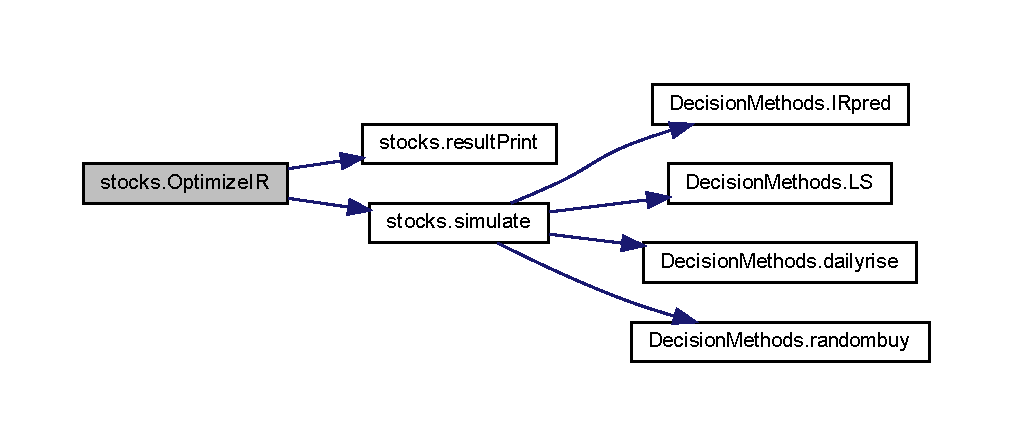
\includegraphics[width=350pt]{namespacestocks_a001673a0b7e5f0867197d97fea8a251b_cgraph}
\end{center}
\end{figure}
\hypertarget{namespacestocks_ac80b7d5d1cdc027b7a0e2e19093baf9b}{}\label{namespacestocks_ac80b7d5d1cdc027b7a0e2e19093baf9b} 
\index{stocks@{stocks}!result\+Print@{result\+Print}}
\index{result\+Print@{result\+Print}!stocks@{stocks}}
\subsubsection{\texorpdfstring{result\+Print()}{resultPrint()}}
{\footnotesize\ttfamily def stocks.\+result\+Print (\begin{DoxyParamCaption}\item[{}]{method,  }\item[{}]{ticker,  }\item[{}]{start,  }\item[{}]{end }\end{DoxyParamCaption})}

\begin{DoxyVerb}Prints results in nice fancy colors
Only tested with bash, but should(?) work for any terminal that
supports bash-like syntax and coloring
\end{DoxyVerb}
 

Definition at line 111 of file stocks.\+py.



Referenced by main(), and Optimize\+I\+R().


\begin{DoxyCode}
111 \textcolor{keyword}{def }\hyperlink{namespacestocks_ac80b7d5d1cdc027b7a0e2e19093baf9b}{resultPrint}(method, ticker, start, end):
112     \textcolor{stringliteral}{"""Prints results in nice fancy colors}
113 \textcolor{stringliteral}{    Only tested with bash, but should(?) work for any terminal that}
114 \textcolor{stringliteral}{    supports bash-like syntax and coloring}
115 \textcolor{stringliteral}{    """}
116     if(start>end):
117         change=\textcolor{stringliteral}{"\(\backslash\)x1b[1;31m \{:2.3f\}% \(\backslash\)x1b[0m"}.format((end-start)/start*100.0)
118     \textcolor{keywordflow}{else}:
119         change=\textcolor{stringliteral}{"\(\backslash\)x1b[1;32m \{:2.3f\}% \(\backslash\)x1b[0m"}.format((end-start)/start*100.0)
120 
121     print(\textcolor{stringliteral}{'\{\} of \{\} starts at \{:3d\}, results in \{:.3f\}. Change:\{\}'}.format(method,ticker,start,end,change))
122 
123 
\end{DoxyCode}
\hypertarget{namespacestocks_a6217dcad564ba6361c3cca44542ba220}{}\label{namespacestocks_a6217dcad564ba6361c3cca44542ba220} 
\index{stocks@{stocks}!simulate@{simulate}}
\index{simulate@{simulate}!stocks@{stocks}}
\subsubsection{\texorpdfstring{simulate()}{simulate()}}
{\footnotesize\ttfamily def stocks.\+simulate (\begin{DoxyParamCaption}\item[{}]{simtype,  }\item[{}]{amount,  }\item[{}]{data,  }\item[{}]{return\+Series = {\ttfamily 0},  }\item[{}]{plot = {\ttfamily 0},  }\item[{}]{extra\+Arg }\end{DoxyParamCaption})}



Definition at line 26 of file stocks.\+py.



References Decision\+Methods.\+dailyrise(), Decision\+Methods.\+I\+Rpred(), Decision\+Methods.\+L\+S(), and Decision\+Methods.\+randombuy().



Referenced by ensemble\+Sim(), main(), and Optimize\+I\+R().


\begin{DoxyCode}
26 \textcolor{keyword}{def }\hyperlink{namespacestocks_a6217dcad564ba6361c3cca44542ba220}{simulate}(simtype, amount, data, returnSeries=0, plot=0, **extraArg):
27     Holding=0
28     Worth=amount
29     startpoint=10
30     WorthSeries=[Worth \textcolor{keywordflow}{for} i \textcolor{keywordflow}{in} range(startpoint)]
31 
32     if(type(data[0]) \textcolor{keywordflow}{is} np.ndarray):
33         X=data[:,0]
34         logging.info(\textcolor{stringliteral}{'Data type is 2d numpy array'})
35     \textcolor{keywordflow}{else}:
36         X=data
37 
38     \textcolor{comment}{#Once you have an idea of the data length, check for date data}
39     date=extraArg.get(\textcolor{stringliteral}{'date'},[i \textcolor{keywordflow}{for} i \textcolor{keywordflow}{in} range(len(X))])
40 
41     \textcolor{comment}{#print(X[-1])}
42 
43     logging.debug(\textcolor{stringliteral}{'len(X): \{0:2d\}'}.format(len(X)))
44 
45     if(plot):
46         f, (ax1, ax2) = plt.subplots(2, sharex=\textcolor{keyword}{True}, figsize=(12, 12), dpi=100)
47 
48     \textcolor{keywordflow}{for} i \textcolor{keywordflow}{in} range(startpoint,len(X)-1):
49         if(type(data[0]) \textcolor{keywordflow}{is} np.ndarray):
50             buysell=simtype(data[0:i+1,:], **extraArg)
51         \textcolor{keywordflow}{else}:
52             buysell=simtype(data[0:i], **extraArg)
53 
54         \textcolor{keywordflow}{if} buysell>0 \textcolor{keywordflow}{and} Holding==0:
55             Holding=floor(Worth/X[i+1])
56             logging.info(\textcolor{stringliteral}{'Buying \{0:3d\} at \{1:.3f\} worth \{2:.3f\}'}.format(Holding,X[i+1],Holding*X[i+1]))
57             if(plot):
58                 ax1.plot(date[i],X[i+1],\textcolor{stringliteral}{'g+'},markersize=10, markeredgewidth=2)
59             Worth-=Holding*X[i+1]
60 
61 
62         \textcolor{keywordflow}{elif} buysell<0 \textcolor{keywordflow}{and} Holding>0:
63             Worth+=Holding*X[i+1]
64             logging.info(\textcolor{stringliteral}{'Selling \{0:3d\}, now worth \{1:.3f\}'}.format(Holding,Worth))
65             Holding=0
66             if(plot):
67                 ax1.plot(date[i],X[i+1],\textcolor{stringliteral}{'r+'},markersize=10, markeredgewidth=2)
68 
69         WorthSeries.append(Worth+Holding*X[i+1])
70 
71 
72     \textcolor{comment}{#Sell off what's left}
73 
74     Worth+=Holding*X[-1]
75     WorthSeries.append(Worth)
76 
77     if(plot):
78         ax1.plot(date,X,\textcolor{stringliteral}{'k'})
79         ax1.set\_ylabel(\textcolor{stringliteral}{'Stock ($)'})
80 
81         ax2.plot(date,WorthSeries, \textcolor{stringliteral}{'k'})
82         ax2.plot(date,[amount \textcolor{keywordflow}{for} i \textcolor{keywordflow}{in} range(len(WorthSeries))],\textcolor{stringliteral}{'r-.'})
83         ax2.set\_ylabel(\textcolor{stringliteral}{'Investment ($)'})
84         ax2.set\_xlabel(\textcolor{stringliteral}{'Day'})
85         f.subplots\_adjust(hspace=0)
86         plt.setp([a.get\_xticklabels() \textcolor{keywordflow}{for} a \textcolor{keywordflow}{in} f.axes[:-1]], visible=\textcolor{keyword}{False})
87         ax1.grid(\textcolor{keyword}{True}, axis=\textcolor{stringliteral}{'x'})
88         ax2.grid(\textcolor{keyword}{True}, axis=\textcolor{stringliteral}{'x'})
89 
90         if(\textcolor{stringliteral}{'ticker'} \textcolor{keywordflow}{in} extraArg):
91             ax1.set\_title(\textcolor{stringliteral}{'Simulating use of \{\} for \{\}'}.format(simtype.\_\_name\_\_,extraArg[\textcolor{stringliteral}{'ticker'}]))
92 
93         \textcolor{comment}{#plt.set\_size\_inches(5, 10)}
94         plt.savefig(\textcolor{stringliteral}{'Plots/\{\}\_\{\}.png'}.format(extraArg[\textcolor{stringliteral}{'ticker'}],simtype.\_\_name\_\_))
95         plt.show()
96 
97     if(returnSeries):
98         \textcolor{keywordflow}{return} WorthSeries
99     \textcolor{keywordflow}{else}:
100         \textcolor{keywordflow}{return} Worth
101 
102     \textcolor{comment}{#Just so the doxygen call graph picks up that these are possible calls}
103     if(0):
104         \hyperlink{namespaceDecisionMethods_a6ee6e338ea6a22bd13d5b9767b126f83}{IRpred}()
105         \hyperlink{namespaceDecisionMethods_a856437b184fc8efd2df5f7fe1ba3644d}{LS}()
106         \hyperlink{namespaceDecisionMethods_a4cb76bf4e82cc2509499af66f8c816b3}{dailyrise}()
107         \hyperlink{namespaceDecisionMethods_a44bd5be577a4d99d6b2d144ad405dd09}{randombuy}()
108 
109 
110 
\end{DoxyCode}
Here is the call graph for this function\+:\nopagebreak
\begin{figure}[H]
\begin{center}
\leavevmode
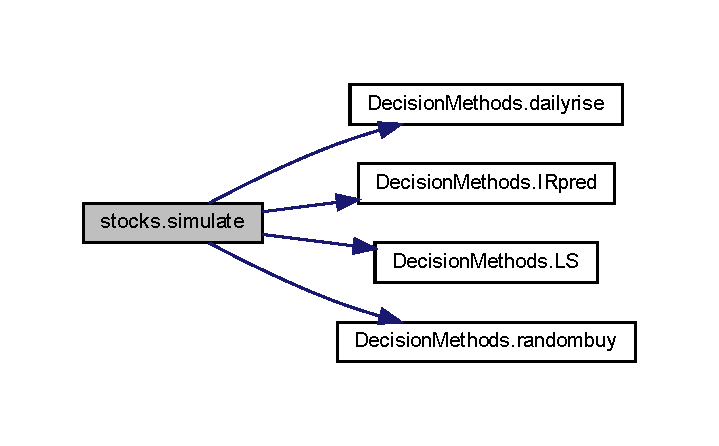
\includegraphics[width=345pt]{namespacestocks_a6217dcad564ba6361c3cca44542ba220_cgraph}
\end{center}
\end{figure}

\chapter{File Documentation}
\hypertarget{DecisionMethods_8py}{}\section{Decision\+Methods.\+py File Reference}
\label{DecisionMethods_8py}\index{Decision\+Methods.\+py@{Decision\+Methods.\+py}}
\subsection*{Namespaces}
\begin{DoxyCompactItemize}
\item 
 \hyperlink{namespaceDecisionMethods}{Decision\+Methods}
\end{DoxyCompactItemize}
\subsection*{Functions}
\begin{DoxyCompactItemize}
\item 
def \hyperlink{namespaceDecisionMethods_a44bd5be577a4d99d6b2d144ad405dd09}{Decision\+Methods.\+randombuy} (data, extra\+Arg)
\item 
def \hyperlink{namespaceDecisionMethods_aed1379cd4db8a24d6e5e45908a88cb4b}{Decision\+Methods.\+weeklyrise} (data, extra\+Arg)
\item 
def \hyperlink{namespaceDecisionMethods_a4cb76bf4e82cc2509499af66f8c816b3}{Decision\+Methods.\+dailyrise} (data, extra\+Arg)
\item 
def \hyperlink{namespaceDecisionMethods_a856437b184fc8efd2df5f7fe1ba3644d}{Decision\+Methods.\+LS} (data, extra\+Arg)
\item 
def \hyperlink{namespaceDecisionMethods_a6ee6e338ea6a22bd13d5b9767b126f83}{Decision\+Methods.\+I\+Rpred} (data, Nx=1, Nf=5, ratio=0.\+03, days=5, extra\+Arg)
\end{DoxyCompactItemize}

\hypertarget{IR_8py}{}\section{I\+R.\+py File Reference}
\label{IR_8py}\index{I\+R.\+py@{I\+R.\+py}}
\subsection*{Namespaces}
\begin{DoxyCompactItemize}
\item 
 \hyperlink{namespaceIR}{IR}
\end{DoxyCompactItemize}
\subsection*{Functions}
\begin{DoxyCompactItemize}
\item 
def \hyperlink{namespaceIR_ae50bbbd323bc928d9e274617de58d72f}{I\+R.\+IR} (X, F, Nx, Nf)
\item 
def \hyperlink{namespaceIR_aeaee615025a0b0c13500382312ba7745}{I\+R.\+verify\+IR} ()
\end{DoxyCompactItemize}

\hypertarget{README_8md}{}\section{R\+E\+A\+D\+M\+E.\+md File Reference}
\label{README_8md}\index{R\+E\+A\+D\+M\+E.\+md@{R\+E\+A\+D\+M\+E.\+md}}

\hypertarget{stocks_8py}{}\section{stocks.\+py File Reference}
\label{stocks_8py}\index{stocks.\+py@{stocks.\+py}}
\subsection*{Namespaces}
\begin{DoxyCompactItemize}
\item 
 \hyperlink{namespacestocks}{stocks}
\end{DoxyCompactItemize}
\subsection*{Functions}
\begin{DoxyCompactItemize}
\item 
def \hyperlink{namespacestocks_a44235135cad9d919663b15452cf3e613}{stocks.\+get\+Closing} (Tick, start=str(date(date.\+today().year-\/1, date.\+today().month, date.\+today().day)), end=str(date.\+today()))
\item 
def \hyperlink{namespacestocks_a6217dcad564ba6361c3cca44542ba220}{stocks.\+simulate} (simtype, amount, data, return\+Series=0, plot=0, extra\+Arg)
\item 
def \hyperlink{namespacestocks_ac80b7d5d1cdc027b7a0e2e19093baf9b}{stocks.\+result\+Print} (method, ticker, start, end)
\item 
def \hyperlink{namespacestocks_a7d4f88b285b7a553f17f91e71ee18a31}{stocks.\+ensemble\+Sim} (simtype, starting\+Worth, data, ticker, ensemble\+Num=100, extra\+Arg)
\item 
def \hyperlink{namespacestocks_a5ce0ea6dd1cb1e1baf78fbb4313b64b9}{stocks.\+Common\+Date} (dateX, X, dateF, F)
\item 
def \hyperlink{namespacestocks_a001673a0b7e5f0867197d97fea8a251b}{stocks.\+Optimize\+IR} (data, starting\+Worth, extra\+Arg)
\item 
def \hyperlink{namespacestocks_aa4d6e539aeea3ab00b8bf598b1025e58}{stocks.\+main} (argv)
\end{DoxyCompactItemize}

%--- End generated contents ---

% Index
\backmatter
\newpage
\phantomsection
\clearemptydoublepage
\addcontentsline{toc}{chapter}{Index}
\printindex

\end{document}
